\chapter{Hardware Accelerator}

The Raspberry Pi 5 with an Ai kit was chosen as the hardware to prove the concept of computing data at the edge.
This desiction was taken based on recommendations from the advisors and the avilability.
The hardware accelerator of the Ai kit is made by Hailo \cite{hailo}.
Hailo is a company which produces hardware accelerators.
The Ai kit uses the Hailo-8L entry level hardware accelerator.
Hailo provides a pipeline to compile a network so that it can be executed on the hailo software.
This pipeline is  called the \Acrfull{dfc}.

\section{Dataflow compiler}

To use the \acrshort{dfc} a pytorch or tensorflow model has to be converted to Onnx or tensorflow light.
Information and pictures are taken from \cite{hailo_dataflow_compiler}.
The \acrshort{dfc} the compiles the model to a \Acrfull{hef} by executing the following steps.
\begin{enumerate}
    \item Tensorflow and ONNX translation
    \item Profiler
    \item Emulator
    \item Model Optimization
    \item Compiling the model into a binary image
\end{enumerate}



\begin{figure}
    \centering
    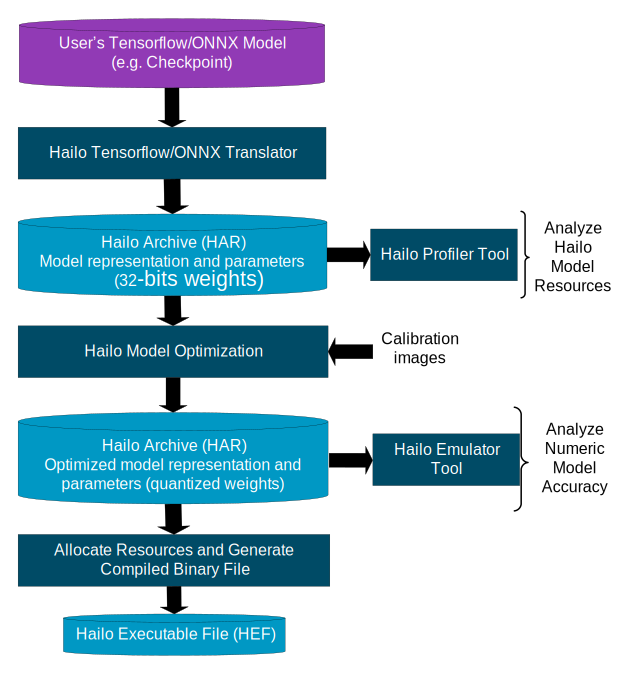
\includegraphics[width=\textwidth]{Images/Hardware/model_build_overview_with_onnx_and_hef_w_har.png}
    \caption{\Acrlong{dfc} overview }
    \label{fig:hardware:dfcoverview}
\end{figure}

\section{Constrains}
At the time of this writing, the \acrshort{dfc} is not capable of compiling Transformers.
Fortunately, the visual encoding of CLIP can also be done with ResNet, a special form of \Acrshort{cnn}.
